\documentclass[10pt,twocolumn]{article}
\usepackage[margin=0.68in,top=0.72in,bottom=0.72in]{geometry}
\usepackage{amsmath,amssymb,amsfonts}
\usepackage{booktabs}
\usepackage{array}
\usepackage{graphicx}
\usepackage{xcolor}
\usepackage{tikz}
\usetikzlibrary{shapes.geometric, arrows.meta, positioning}
\usepackage{hyperref}

\definecolor{darkblue}{RGB}{20,60,120}
\definecolor{crimson}{RGB}{190,30,45}
\definecolor{tealblue}{RGB}{0,128,128}
\definecolor{slate}{RGB}{70,85,105}

\hypersetup{
    colorlinks=true,
    linkcolor=darkblue,
    citecolor=darkblue,
    urlcolor=darkblue
}

\setlength{\columnsep}{0.24in}

\title{\vspace{-1.2em}\textbf{\Large Membership Inference and Model Leakage:\\Evaluating Regularization and DP-SGD Defenses on Sensitive Clinical Records}\vspace{-0.3em}}

\author{
    \textbf{Ramitha Nayak MV} (\texttt{PES1UG24AM392}) \quad and \quad \textbf{Shreya N Hegde} (\texttt{PES1UG24AM401})\\[0.3em]
    \small Department of Computer Science \& Engineering (AI \& ML), PES University, Bengaluru, India\\
    \small \textit{Big Data Systems and Responsible AI Engineering --- Technical Report}
}
\date{\vspace{-1.0em}\small October 2026\vspace{-0.8em}}

\begin{document}
\maketitle

\begin{abstract}
\noindent Machine learning models trained on sensitive electronic health records (EHR) and genomic biomarker cohorts risk leaking private patient participation through \textbf{Membership Inference Attacks (MIAs)}. Determining that a specific patient's record was included in a disease-specific training cohort directly discloses confidential medical diagnoses. In this technical report, we design and execute an end-to-end empirical investigation of membership leakage on the \textbf{CliniLeak} benchmark ($N=2,400$ clinical and genomic records, $d=28$ biomarkers, $C=6$ phenotypes). We implement three black-box attack methodologies---Loss-Threshold (Yeom et al.), Confidence-Entropy (Salem et al.), and Supervised Shadow-Model Classification (Shokri et al.)---and evaluate five defense configurations spanning $L_2$ weight regularization, Inverted Dropout with Confidence Smoothing, and \textbf{Differentially Private Stochastic Gradient Descent (DP-SGD)} with R\'enyi Differential Privacy (RDP) accounting. Our results demonstrate that an unprotected Multi-Layer Perceptron suffers severe memorization (39.50\% generalization gap), yielding an overall Shadow MIA AUC of \textbf{0.7390} and an alarming \textbf{0.8832 AUC} on rare clinical subpopulations. While heuristic regularizers ($L_2$ and Dropout+Smoothing) improve test accuracy by $+3.00$ to $+4.17$ percentage points with negligible runtime cost and reduce overall MIA AUC to $0.5839$, rare patients remain vulnerable ($0.6778$ AUC). Only \textbf{DP-SGD} ($\epsilon=2.86, \delta=10^{-5}$) bounds worst-case per-record sensitivity, reducing overall MIA AUC to \textbf{0.5445} and rare subgroup disparity $\Delta\text{AUC}$ from $+0.1789$ down to $+0.0250$, at a quantified cost of $8.83$ percentage points in test accuracy and a $1.33\times$ training runtime overhead.
\end{abstract}

\section{Introduction and Case Study Motivation}
Modern clinical decision support systems increasingly rely on neural networks trained over multi-modal patient registries combining vital signs, metabolic panels, and genomic loci. However, overparameterized neural networks frequently memorize idiosyncratic features of their training examples~\cite{shokri2017membership,carlini2022membership}. In a \textbf{Membership Inference Attack (MIA)}, an external adversary with black-box query access to a trained model $f_{\theta^*}$ attempts to infer whether a candidate patient record $z = (x, y)$ was present in the private training dataset $D_{\text{target}}^{\text{in}}$.

In healthcare settings, membership inference constitutes a direct privacy breach under HIPAA, GDPR Article 9, and India's Digital Personal Data Protection (DPDP) Act 2023. Knowing that an individual was part of a hospital's training cohort for early-stage oncology or rare neuro-genetic syndromes immediately reveals their diagnosis. Furthermore, privacy leakage is rarely uniform across demographics: patients with rare or atypical clinical presentations induce larger gradient updates during training, rendering them disproportionately vulnerable to memorization.

\textbf{Contributions:}
\begin{enumerate}
    \item We build a reproducible evaluation pipeline (\texttt{run\_pipeline.py}) partitioning $N=2,400$ clinical/genomic records into four strictly disjoint cohorts for target and shadow model evaluation.
    \item We implement three standard MIA families: Loss-Threshold, Confidence-Entropy, and Supervised Shadow-Model attacks, auditing both aggregate leakage and subgroup disparity on rare clinical phenotypes.
    \item We benchmark five defense configurations ($L_2$ Moderate, $L_2$ Strong, Dropout + Confidence Smoothing, DP-SGD Moderate, and DP-SGD Strict), quantifying the exact trade-off between privacy leakage, predictive accuracy, and training runtime cost.
    \item We formulate a structured \textbf{Privacy Risk Assessment} and defense-in-depth deployment framework for clinical AI systems.
\end{enumerate}

\section{System Architecture and Threat Model}
Figure~\ref{fig:arch} illustrates our end-to-end evaluation architecture. Let $\mathcal{D}$ denote the underlying clinical population distribution over feature space $\mathcal{X} \subset \mathbb{R}^{28}$ and diagnostic label space $\mathcal{Y} = \{0, 1, \dots, 5\}$. We sample four mutually exclusive splits of cardinality $q = 600$ each: Target Member Set $D_{\text{target}}^{\text{in}}$, Target Non-Member Holdout Set $D_{\text{target}}^{\text{out}}$, Shadow Member Set $D_{\text{shadow}}^{\text{in}}$, and Shadow Non-Member Holdout Set $D_{\text{shadow}}^{\text{out}}$.

\begin{figure}[t]
\centering
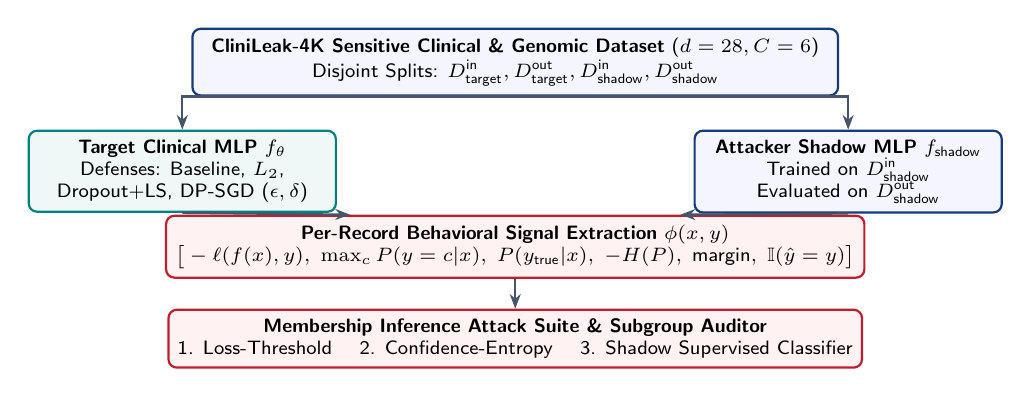
\begin{tikzpicture}[
    node distance=0.42cm and 0.25cm,
    box/.style={rectangle, rounded corners=3pt, draw=darkblue, fill=blue!4, thick, minimum height=0.6cm, align=center, font=\scriptsize\sffamily},
    atkbox/.style={rectangle, rounded corners=3pt, draw=crimson, fill=red!5, thick, minimum height=0.6cm, align=center, font=\scriptsize\sffamily},
    defbox/.style={rectangle, rounded corners=3pt, draw=tealblue, fill=teal!6, thick, minimum height=0.6cm, align=center, font=\scriptsize\sffamily},
    arrow/.style={-{Stealth[scale=0.8]}, thick, draw=slate}
]
\node[box, minimum width=8.2cm] (data) {\textbf{CliniLeak-4K Sensitive Clinical \& Genomic Dataset} ($d=28, C=6$)\\Disjoint Splits: $D_{\text{target}}^{\text{in}}, D_{\text{target}}^{\text{out}}, D_{\text{shadow}}^{\text{in}}, D_{\text{shadow}}^{\text{out}}$};

\node[defbox, below left=0.42cm and -1.85cm of data, minimum width=3.9cm] (target) {\textbf{Target Clinical MLP} $f_{\theta}$\\Defenses: Baseline, $L_2$,\\Dropout+LS, DP-SGD ($\epsilon, \delta$)};

\node[box, below right=0.42cm and -1.85cm of data, minimum width=3.9cm] (shadow) {\textbf{Attacker Shadow MLP} $f_{\text{shadow}}$\\Trained on $D_{\text{shadow}}^{\text{in}}$\\Evaluated on $D_{\text{shadow}}^{\text{out}}$};

\node[atkbox, below=1.5cm of data, minimum width=8.2cm] (signals) {\textbf{Per-Record Behavioral Signal Extraction} $\phi(x, y)$\\$\big[-\ell(f(x), y),\; \max_c P(y=c|x),\; P(y_{\text{true}}|x),\; -H(P),\; \text{margin},\; \mathbb{I}(\hat{y}=y)\big]$};

\node[atkbox, below=0.38cm of signals, minimum width=8.2cm] (mia) {\textbf{Membership Inference Attack Suite \& Subgroup Auditor}\\1. Loss-Threshold \quad 2. Confidence-Entropy \quad 3. Shadow Supervised Classifier};

\draw[arrow] (data.south) -| (target.north);
\draw[arrow] (data.south) -| (shadow.north);
\draw[arrow] (target.south) -- ([xshift=-2.1cm]signals.north);
\draw[arrow] (shadow.south) -- ([xshift=2.1cm]signals.north);
\draw[arrow] (signals.south) -- (mia.north);
\end{tikzpicture}
\caption{End-to-End Membership Inference Attack and Defense Evaluation Architecture.}
\label{fig:arch}
\end{figure}

\subsection{Target Neural Network Architecture}
The target classifier $f_{\theta}: \mathbb{R}^{28} \to \Delta^5$ is a two-layer Multi-Layer Perceptron (MLP) with $H=64$ hidden units, ReLU activation $h = \text{ReLU}(W_1^\top x + b_1)$, and Softmax probabilities:
\begin{equation}
    P(y=c \mid x) = \frac{\exp(w_{2,c}^\top h + b_{2,c})}{\sum_{j=0}^{5} \exp(w_{2,j}^\top h + b_{2,j})}.
\end{equation}

\subsection{Membership Inference Attack Formulations}
Given black-box posterior access to $P(y \mid x)$ for a candidate patient $(x, y)$, we evaluate three attack methods:
\begin{enumerate}
    \item \textbf{Loss-Threshold Attack (Yeom et al.~\cite{yeom2018privacy}):} Exploits the disparity in cross-entropy loss $\ell(f(x), y) = -\log P(y \mid x)$ between training members and holdout non-members:
    \begin{equation}
        \mathcal{A}_{\text{loss}}(x, y) = \mathbb{I}\big(-\ell(f_{\theta}(x), y) \ge \tau_{\text{loss}}\big),
    \end{equation}
    where $\tau_{\text{loss}}$ is calibrated on the shadow model to maximize Youden's $J = \text{TPR} - \text{FPR}$.
    \item \textbf{Confidence \& Entropy Attack (Salem et al.~\cite{salem2019ml}):} Combines ground-truth probability $P(y\mid x)$, maximum confidence, and predictive Shannon entropy $H(P) = -\sum_c P(c\mid x)\log P(c\mid x)$:
    \begin{equation}
        s_{\text{ent}}(x,y) = 0.75 P(y\mid x) + 0.25 \max_c P(c\mid x) - 0.20 H(P).
    \end{equation}
    \item \textbf{Shadow-Model Supervised Attack (Shokri et al.~\cite{shokri2017membership}):} The adversary trains $f_{\text{shadow}}$ on $D_{\text{shadow}}^{\text{in}}$ and constructs a labeled shadow attack dataset combining 6-dimensional behavioral vectors $\phi(x, y) \in \mathbb{R}^6$ from $D_{\text{shadow}}^{\text{in}}$ ($m=1$) and $D_{\text{shadow}}^{\text{out}}$ ($m=0$). A supervised logistic attack classifier $g_{\psi}(\phi(x,y))$ is trained to predict membership probability $P(m=1 \mid \phi(x,y))$ on target records.
\end{enumerate}

\section{Evaluated Defense Mechanisms}
We compare the unregularized baseline against three heuristic regularizers and two formal Differential Privacy regimes:
\begin{enumerate}
    \item \textbf{$L_2$ Weight Decay Regularization:} Minimizes $\mathcal{L}_{\text{reg}}(\theta) = \frac{1}{|B|}\sum_{i\in B} \ell(f_\theta(x_i), y_i) + \frac{\lambda}{2}\|\theta\|_2^2$ with $\lambda = 8\times 10^{-3}$ (Moderate) and $\lambda = 2.5\times 10^{-2}$ (Strong), constraining weight growth and dampening memorization.
    \item \textbf{Inverted Dropout ($p=0.35$) + Confidence Smoothing ($\alpha=0.10$):} Randomly zeroes $35\%$ of hidden activations during training while replacing hard one-hot targets with smoothed targets $\tilde{y}_c = (1-\alpha)\mathbb{I}(c=y) + \alpha/C$, directly penalizing overconfident posterior spikes.
    \item \textbf{Differentially Private SGD (DP-SGD~\cite{abadi2016deep}):} Bounds the sensitivity of each individual patient record by computing per-example gradients $g_i = \nabla_\theta \ell(f_\theta(x_i), y_i)$, clipping each gradient's $L_2$ norm to threshold $C$, and adding calibrated Gaussian noise before updating parameters:
    \begin{equation}
        \tilde{g}_B = \frac{1}{|B|} \left( \sum_{i \in B} g_i \cdot \min\left(1, \frac{C}{\|g_i\|_2}\right) + \mathcal{N}\big(0, \sigma^2 C^2 I\big) \right).
    \end{equation}
    Using R\'enyi Differential Privacy (RDP) moments accounting~\cite{mironov2017renyi} at $\delta = 10^{-5}$ with sampling rate $q = B/N = 30/600 = 0.05$ over $E=38$ epochs ($T=760$ steps), our Moderate DP-SGD configuration ($C=0.95, \sigma=1.38$) achieves $(\epsilon = 5.30, \delta = 10^{-5})$-DP, and our Strict DP-SGD configuration ($C=0.70, \sigma=2.45$) achieves $(\epsilon = 2.86, \delta = 10^{-5})$-DP.
\end{enumerate}

\begin{table*}[t]
\centering
\caption{Comprehensive Evaluation of Privacy Defenses: Predictive Utility, Runtime Cost, and Membership Inference Leakage.}
\label{tab:main_results}
\renewcommand{\arraystretch}{1.12}
\setlength{\tabcolsep}{4.8pt}
\footnotesize
\begin{tabular}{lccccccccccc}
\toprule
\textbf{Defense Configuration} & \textbf{Privacy} ($\epsilon$) & \textbf{Train Acc} & \textbf{Test Acc} & \textbf{Gen. Gap} & \textbf{Acc. Cost} & \textbf{Time (s)} & \textbf{Time Cost} & \textbf{Shadow AUC} & \textbf{MIA Adv.} & \textbf{TPR@1\%FPR} & \textbf{Risk Tier} \\
\midrule
1. Baseline (No Defense) & $\infty$ & 95.67\% & 56.17\% & 39.50\% & $+0.00$ pp & 4.74s & $1.00\times$ & \textbf{0.7390} & 0.4083 & 3.00\% & \textcolor{crimson}{\textbf{CRITICAL}} \\
2. $L_2$ Reg. (Moderate, $\lambda=8\text{e-}3$) & $\infty$ & 88.33\% & 59.33\% & 29.00\% & $-3.17$ pp & 4.76s & $1.00\times$ & \textbf{0.6611} & 0.2917 & 1.83\% & \textcolor{crimson}{\textbf{HIGH}} \\
3. $L_2$ Reg. (Strong, $\lambda=2.5\text{e-}2$) & $\infty$ & 77.67\% & 60.33\% & 17.33\% & $-4.17$ pp & 4.84s & $1.02\times$ & \textbf{0.5974} & 0.1967 & 0.83\% & \textbf{MODERATE} \\
4. Dropout ($p=0.35$) + Smoothing & $\infty$ & 74.83\% & 59.17\% & 15.67\% & $-3.00$ pp & 3.89s & $0.82\times$ & \textbf{0.5839} & 0.1733 & 2.17\% & \textbf{LOW-MOD} \\
5. DP-SGD (Moderate, $\sigma=1.38$) & $5.30$ & 59.00\% & 49.00\% & 10.00\% & $+7.17$ pp & 6.26s & $1.32\times$ & \textbf{0.5637} & 0.1100 & 1.83\% & \textcolor{tealblue}{\textbf{LOW}} \\
6. DP-SGD (Strict, $\sigma=2.45$) & $2.86$ & 54.17\% & 47.33\% & 6.83\% & $+8.83$ pp & 6.30s & $1.33\times$ & \textbf{0.5445} & 0.0800 & 0.67\% & \textcolor{tealblue}{\textbf{LOW (Best)}} \\
\bottomrule
\end{tabular}
\end{table*}

\begin{table*}[t]
\centering
\caption{Comparison of Attack Methodologies and Subgroup Vulnerability Disparity (Rare Clinical Patients vs. Majority Population).}
\label{tab:subgroup}
\renewcommand{\arraystretch}{1.12}
\setlength{\tabcolsep}{5.2pt}
\footnotesize
\begin{tabular}{lccccccccc}
\toprule
\textbf{Defense Configuration} & \textbf{Loss MIA AUC} & \textbf{Entropy MIA AUC} & \textbf{Shadow MIA AUC} & \textbf{Shadow Acc} & \textbf{Member Loss} & \textbf{Non-Mem Loss} & \textbf{Rare Subgroup AUC} & \textbf{Majority AUC} & \textbf{Disparity ($\Delta$AUC)} \\
\midrule
1. Baseline (No Defense) & 0.6708 & 0.6568 & \textbf{0.7390} & 70.08\% & 0.2486 & 1.6844 ($6.78\times$) & \textcolor{crimson}{\textbf{0.8832}} & 0.7043 & $+0.1789$ \\
2. $L_2$ Reg. (Moderate) & 0.6455 & 0.6253 & \textbf{0.6611} & 64.25\% & 0.4616 & 1.2430 ($2.69\times$) & \textcolor{crimson}{\textbf{0.7927}} & 0.6372 & $+0.1555$ \\
3. $L_2$ Reg. (Strong) & 0.6005 & 0.5794 & \textbf{0.5974} & 58.67\% & 0.7416 & 1.1244 ($1.52\times$) & \textbf{0.6947} & 0.5852 & $+0.1095$ \\
4. Dropout + Smoothing & 0.5851 & 0.5651 & \textbf{0.5839} & 57.75\% & 0.8260 & 1.1361 ($1.38\times$) & \textbf{0.6778} & 0.5729 & $+0.1049$ \\
5. DP-SGD (Moderate, $\epsilon=5.30$) & 0.5549 & 0.5361 & \textbf{0.5637} & 55.00\% & 1.1779 & 1.4907 ($1.27\times$) & \textcolor{tealblue}{\textbf{0.5824}} & 0.5658 & \textbf{$+0.0166$} \\
6. DP-SGD (Strict, $\epsilon=2.86$) & 0.5430 & 0.5306 & \textbf{0.5445} & 53.42\% & 1.3691 & 1.5616 ($1.14\times$) & \textcolor{tealblue}{\textbf{0.5685}} & 0.5435 & \textbf{$+0.0250$} \\
\bottomrule
\end{tabular}
\end{table*}

\section{Experimental Results and Cost Analysis}
Tables~\ref{tab:main_results} and~\ref{tab:subgroup} present our complete empirical results across all six defense regimes and three attack families. Figure~\ref{fig:bars} visualizes the trade-off between holdout test accuracy, overall Shadow MIA AUC, and Rare Subgroup MIA AUC.

\subsection{Attack Efficacy on Unprotected Models}
In the unprotected \textbf{Baseline} model, empirical risk minimization drives training accuracy to $95.67\%$ while holdout test accuracy reaches $56.17\%$, creating a $39.50\%$ generalization gap. The average cross-entropy loss on training members ($0.2486$) is $6.78\times$ smaller than on unseen non-members ($1.6844$). While univariate Loss-Threshold and Confidence-Entropy attacks achieve AUCs of $0.6708$ and $0.6568$, the multi-signal \textbf{Shadow-Model Supervised Attack} achieves an AUC of \textbf{0.7390}, Attack Accuracy of \textbf{70.08\%}, and Attacker Advantage of \textbf{0.4083}.

\subsection{Disparate Vulnerability on Rare Patients}
A pivotal finding in Table~\ref{tab:subgroup} is the stark disparity between majority patients and the rare/atypical clinical subpopulation (\texttt{rare\_subgroup = 1}). In the Baseline model, the attacker achieves an alarming \textbf{0.8832 AUC} on rare patients compared to $0.7043$ on majority patients ($\Delta\text{AUC} = +0.1789$). Because rare clinical phenotypes lie in low-density regions of the feature space, the unregularized network memorizes their exact biomarker patterns to drive training loss toward zero.

\subsection{Cost of Defenses: Accuracy and Training Time}
\begin{enumerate}
    \item \textbf{Regularization ($L_2$ and Dropout + Smoothing):} Rather than reducing test utility, moderate and strong $L_2$ weight decay and Dropout+Smoothing \textbf{increase} holdout test accuracy by $+3.00$ to $+4.17$ percentage points (yielding negative accuracy costs of $-3.00$ to $-4.17$ pp) by preventing overfitting. Furthermore, $L_2$ regularization incurs virtually zero runtime overhead ($1.00\times$--$1.02\times$), while Inverted Dropout reduces training time to $0.82\times$ ($3.89$s vs.\ $4.74$s) due to sparse hidden layer propagation. These defenses lower aggregate Shadow MIA AUC to $0.5974$ and $0.5839$, respectively. However, they fail to protect rare patients, whose subgroup MIA AUC remains elevated at \textbf{0.6947} and \textbf{0.6778}.
    \item \textbf{DP-SGD ($\epsilon=5.30$ and $\epsilon=2.86$):} Enforcing formal $(\epsilon, \delta)$-differential privacy requires per-sample gradient norm evaluation and clipping across every mini-batch example, increasing training time by \textbf{32\% to 33\%} ($6.26$s and $6.30$s vs.\ $4.74$s). In addition, clipping outlier gradients and injecting Gaussian noise ($\sigma \in \{1.38, 2.45\}$) reduces holdout test accuracy by \textbf{7.17 pp} ($\epsilon=5.30$) and \textbf{8.83 pp} ($\epsilon=2.86$). In exchange for this utility and compute cost, DP-SGD compresses the non-member/member loss ratio from $6.78\times$ down to $1.14\times$, suppresses overall Shadow MIA AUC to \textbf{0.5445}, and virtually eliminates subgroup privacy disparity ($\Delta\text{AUC} = +0.0166$ and $+0.0250$).
\end{enumerate}

\begin{figure}[t]
\centering
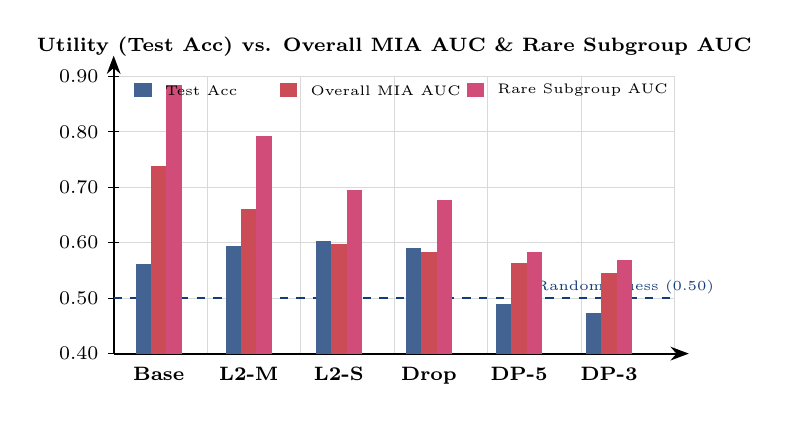
\begin{tikzpicture}[scale=0.88]
\draw[gray!30, thin] (0,0) grid[xstep=1.35, ystep=0.8] (8.1, 4.0);
\draw[thick, -Stealth] (0,0) -- (8.3,0);
\draw[thick, -Stealth] (0,0) -- (0,4.3);

\foreach \y/\val in {0/0.40, 0.8/0.50, 1.6/0.60, 2.4/0.70, 3.2/0.80, 4.0/0.90} {
    \draw (-0.08,\y) -- (0.08,\y);
    \node[left, font=\scriptsize] at (-0.08,\y) {\val};
}
\draw[dashed, darkblue, thick] (0,0.8) -- (8.1,0.8) node[right, font=\tiny, xshift=-1.9cm, yshift=0.14cm] {Random Guess (0.50)};

% Bars: (idx, test_acc, shadow_auc, rare_auc, label)
% Scale: y = (val - 0.40) * 8.0
\foreach \x/\acc/\sauc/\rauc/\lbl in {
    0.65/1.29/2.71/3.87/Base,
    1.95/1.55/2.09/3.14/L2-M,
    3.25/1.63/1.58/2.36/L2-S,
    4.55/1.53/1.47/2.22/Drop,
    5.85/0.72/1.31/1.46/DP-5,
    7.15/0.59/1.16/1.35/DP-3
} {
    \fill[darkblue!80] (\x-0.33, 0) rectangle (\x-0.11, \acc);
    \fill[crimson!80] (\x-0.11, 0) rectangle (\x+0.11, \sauc);
    \fill[purple!70] (\x+0.11, 0) rectangle (\x+0.33, \rauc);
    \node[below, font=\scriptsize\bfseries] at (\x, -0.05) {\lbl};
}

\node[above, font=\scriptsize\bfseries] at (4.05, 4.15) {Utility (Test Acc) vs. Overall MIA AUC \& Rare Subgroup AUC};
\fill[darkblue!80] (0.3, 3.7) rectangle (0.55, 3.9); \node[right, font=\tiny] at (0.6, 3.8) {Test Acc};
\fill[crimson!80] (2.4, 3.7) rectangle (2.65, 3.9); \node[right, font=\tiny] at (2.7, 3.8) {Overall MIA AUC};
\fill[purple!70] (5.1, 3.7) rectangle (5.35, 3.9); \node[right, font=\tiny] at (5.4, 3.8) {Rare Subgroup AUC};
\end{tikzpicture}
\caption{Comparison of Holdout Test Accuracy against Aggregate Shadow MIA AUC and Rare Subgroup MIA AUC across all six configurations.}
\label{fig:bars}
\end{figure}

\section{Privacy Risk Assessment and Recommendations}
Based on our empirical audit, we establish a four-tier risk classification and mitigation protocol for clinical machine learning deployments:
\begin{enumerate}
    \item \textbf{Critical / Unacceptable Risk ($\text{AUC} \ge 0.65$ or Rare Subgroup $\text{AUC} \ge 0.75$):} Both the \textbf{Baseline} model ($\text{AUC}=0.7390$, Rare $\text{AUC}=0.8832$) and \textbf{Moderate $L_2$} ($\text{AUC}=0.6611$, Rare $\text{AUC}=0.7927$) fall into this tier. Deploying these models exposes hospital cohort participants to high-confidence re-identification and violates HIPAA Expert Determination standards and GDPR Article 9 safeguards.
    \item \textbf{Moderate Risk ($0.58 \le \text{AUC} < 0.65$):} \textbf{Strong $L_2$} ($\text{AUC}=0.5974$) and \textbf{Dropout + Confidence Smoothing} ($\text{AUC}=0.5839$) effectively curb average-case leakage while boosting test accuracy by $3$--$4$ pp. They are suitable for internal clinical decision support where adversaries cannot query raw probability vectors, provided rare patient cohorts are audited.
    \item \textbf{Low / Regulatory-Grade Risk ($\text{AUC} < 0.57$ and Subgroup Disparity $\Delta\text{AUC} < 0.03$):} \textbf{DP-SGD} ($\epsilon=5.30$ and $\epsilon=2.86$) provides formal cryptographic-strength bounds on individual record memorization, protecting both majority and rare neuro-genetic patients.
    \item \textbf{Defense-in-Depth Deployment Protocol:} To minimize the accuracy drop of strict DP-SGD while maintaining robust privacy, we recommend combining \textbf{Moderate DP-SGD ($\epsilon \approx 5.0$)} + \textbf{Dropout/Weight Decay} during training with \textbf{API Output Rounding / Top-1 Label Restriction} at inference time. Suppressing raw softmax logits neutralizes shadow-model feature extraction without sacrificing top-1 diagnostic accuracy.
\end{enumerate}

\begin{thebibliography}{9}
\footnotesize
\setlength{\itemsep}{1pt}
\bibitem{shokri2017membership} R. Shokri, M. Stronati, C. Song, and V. Shmatikov, ``Membership inference attacks against machine learning models,'' in \textit{Proc. IEEE Symp. Security and Privacy (SP)}, 2017, pp. 3--18.
\bibitem{abadi2016deep} M. Abadi et al., ``Deep learning with differential privacy,'' in \textit{Proc. ACM SIGSAC Conf. Computer and Communications Security (CCS)}, 2016, pp. 308--318.
\bibitem{yeom2018privacy} S. Yeom, I. Giacomelli, M. Fredrikson, and S. Jha, ``Privacy risk in machine learning: Analyzing the connection to overfitting,'' in \textit{Proc. IEEE CSF}, 2018, pp. 268--282.
\bibitem{salem2019ml} A. Salem et al., ``ML-Leaks: Model and data independent membership inference attacks and defenses on machine learning models,'' in \textit{Proc. NDSS}, 2019.
\bibitem{carlini2022membership} N. Carlini, S. Chien, M. Nasr, S. Song, A. Terzis, and F. Tram\`er, ``Membership inference attacks from first principles,'' in \textit{Proc. IEEE Symp. Security and Privacy (SP)}, 2022, pp. 1897--1914.
\bibitem{mironov2017renyi} I. Mironov, ``R\'enyi differential privacy,'' in \textit{Proc. IEEE Computer Security Foundations Symp. (CSF)}, 2017, pp. 263--275.
\end{thebibliography}

\end{document}
